\section{Contributions}
\label{sec:contributions}

\subsection{Recurrent Clustering}
\label{sec:recurrentclustering}

\iffalse TODO: Focus the section more on the problem of identifiers, and how recurrent clustering uses clustering as part of feature extraction to solve this \fi

We adapt the methodology of \emph{recurrent clustering} proposed in \citep{DBLP:journals/corr/HerasK14, heras2013proof}, and suggest a new recurrent clustering and feature extraction algorithm for Haskell \iffalse TODO: Fix the end of this sentence \fi theory exploration. As a clustering algorithm, the aim of recurrent clustering is to identify similarities in a set of data points (in our case, Core expressions). Its distinguishing characteristic is to \emph{combine} feature extraction and clustering into a single recursive algorithm (shown as algorithm \ref{alg:recurrent}), which goes beyond a simple syntactic characterisation, to allow the features of an expression to depend on those it references. Here we describe our approach to recurrent clustering and compare its similarity and differences to those of ML4PG and ACL2(ml).

We consider our algorithm in two stages: the first transforms the nested structure of expressions into a flat feature vector representation; the second converts the discrete symbols of Core syntax into features (real numbers), which we will denote using the notation $\feature{}$.

\subsubsection{Expressions to Vectors}

Our recurrent clustering algorithm makes use of the k-means algorithm described in \S \ref{sec:kmeans}, which considers the elements of a feature vector to be \emph{orthogonal}. Hence we must ensure that similar expressions not only give rise to similar numerical values, but crucially that these values appear \emph{at the same position} in the feature vectors. Since different patterns of nesting can alter the ``shape'' of expressions, simple traversals (breadth-first, depth-first, post-order, etc.) may cause features from equivalent sub-expressions to be mis-aligned. For example, consider the following expressions, which represent pattern-match clauses with different patterns but the same body (\hs{\vlocal{y}}):

\begin{equation*}
  \begin{array}{r@{}l@{}l@{}}
    X\ &=\ \CAlt\ (\CDataAlt\ \id{C})\ & (\vlocal{y}) \\
    Y\ &=\ \CAlt\ \CDefault\           & (\vlocal{y})
  \end{array}
\end{equation*}

If we traverse these expressions in breadth-first order, converting each token to a feature using $\feature{}$ and padding to the same length with $0$, we would get the following feature vectors:

\begin{small}
  \begin{equation*}
    \begin{array}{r@{}l@{}l@{}l@{}l@{}l@{}l@{}l}
      breadthFirst(X)\ &=\ (\feature{\CAlt},\ &\feature{\CDataAlt},\ &\feature{\CVar},\ &\feature{\id{C}},\ &\feature{\CLocal},\ &\feature{\id{y}} &) \\
      breadthFirst(Y)\ &=\ (\feature{\CAlt},\ &\feature{\CDefault},\ &\feature{\CVar},\ &\feature{\CLocal},\ &\feature{\id{y}},\ &0 &)
    \end{array}
  \end{equation*}
\end{small}

Here the features corresponding to the common sub-expression $\CLocal\ \id{y}$ are misaligned, such that only $\frac{1}{3}$ of features are guaranteed to match (others may match by coincidence, depending on $\feature{}$). These feature vectors might be deemed very dissimilar during clustering, despite the intuitive similarity of the expressions $X$ and $Y$ from which they derive.

If we were to align these feature optimally, by padding the fourth column rather than the sixth, then $\frac{2}{3}$ of features would be guaranteed to match, making the similarity of the vectors more closely match our intuition and depend less on coincidence.

The method we use to ``flatten'' expressions, described below, is a variation of breadth-first traversal which pads each level of nesting to a fixed size $c$ (for \emph{columns}). This doesn't guarantee alignment, but it does prevent mis-alignment from accumulating across different levels of nesting. Our method would align these features into the following vectors, if $c = 2$: \footnote{In fact, the $toTree$ function would ignore the constructor identifier $\id{C}$ and never produce the feature $\feature{\id{C}}$. However, this example is still accurate in terms of laying out the features as given.}

\begin{small}
  \begin{equation*}\label{eq:flattened}
    \begin{array}{r@{}l@{}l@{}l@{}l@{}l@{}l@{}l@{}l@{}l}
      featureVec(X)\ &=\ (\feature{\CAlt},\ &0,\ &\feature{\CDataAlt},\ &\feature{\CVar},\ &\feature{\id{C}},\  &\feature{\CLocal},\ &\feature{\id{y}},\ &0 &) \\
      featureVec(Y)\ &=\ (\feature{\CAlt},\ &0,\ &\feature{\CDefault},\ &\feature{\CVar},\ &\feature{\CLocal},\ &0,\                 &\feature{\id{y}},\ &0 &)
    \end{array}
  \end{equation*}
\end{small}

Here $\frac{1}{2}$ of the original 6 features align, which is more than $breadthFirst$ but not optimal. Both vectors have also been padded by an extra 2 zeros compared to $breadthFirst$; raising their alignment to $\frac{5}{8}$.

To perform this flattening we first transform the nested tokens of an expression into a \emph{rose tree} of features, using the $toTree$ function shown in Figure \ref{fig:totree}. \iffalse TODO: Make a formal definition in an environment, i.e. not inline? \fi Rose trees are defined recursively: $T$ is a rose tree if $T = (f, T_1, \dots, T_{n_T})$, where $f \in \mathbb{R}$ and $T_i$ are rose trees. $T_i$ are the \emph{sub-trees} of $T$ and $f$ is the \emph{feature at} $T$. $n_T$ may differ for each (sub-) tree; trees where $n_T = 0$ are \emph{leaves}. The results are illustrated in Figure \ref{fig:rosetreeexample}.

\begin{figure}
  \begin{align*}
    toTree(e) &=
    \begin{cases}
      (\feature{\CVar},     toTree(e_1))                                 & \text{if $e = \CVar\ e_1$} \\
      (\feature{\CLit},     toTree(e_1))                                 & \text{if $e = \CLit\ e_1$} \\
      (\feature{\CApp},     toTree(e_1), toTree(e_2))                    & \text{if $e = \CApp\ e_1\ e_2$} \\
      (\feature{\CLam},     toTree(e_1))                                 & \text{if $e = \CLam\ l_1\ e_1$} \\
      (\feature{\CLet},     toTree(e_1), toTree(e_2))                    & \text{if $e = \CLet\ e_1\ e_2$} \\
      (\feature{\CCase},    toTree(e_1), toTree(a_1), \dots)             & \text{if $e = \CCase\ e_1\ l_1 a_1 \dots$} \\
      (\feature{\CType})                                                & \text{if $e = \CType$} \\
      (\feature{\CLocal},   leaf(l_1))                                  & \text{if $e = \CLocal\ l_1$} \\
      (\feature{\CGlobal},  leaf(g_1))                                  & \text{if $e = \CGlobal\ g_1$} \\
      (\feature{\CConstructor})                                         & \text{if $e = \CConstructor\ d_1$} \\
      (\feature{\CLitNum})                                              & \text{if $e = \CLitNum\ n_1$} \\
      (\feature{\CLitStr})                                              & \text{if $e = \CLitStr\ s_1$} \\
      (\feature{\CAlt},     toTree(e_1), toTree(e_2))                   & \text{if $e = \CAlt\ e_1 e_2 l_1 \dots$}  \\
      (\feature{\CDataAlt})                                             & \text{if $e = \CDataAlt\ g_1$}  \\
      (\feature{\CLitAlt},  toTree(e_1))                                & \text{if $e = \CLitAlt\ e_1$}  \\
      (\feature{\CDefault})                                             & \text{if $e = \CDefault$}  \\
      (\feature{\CNonRec},  toTree(e_1))                                & \text{if $e = \CNonRec\ e_1$}  \\
      (\feature{\CRec},     toTree(e_1), \dots)                         & \text{if $e = \CRec\ e_1 \dots$} \\
      (\feature{\CBind},    toTree(e_1))                                & \text{if $e = \CBind\ l_1 e_1$}
    \end{cases} \\
    leaf(x) &= (\feature{x}) \iffalse TODO: This is completely unnecessary... \fi
  \end{align*}
  \caption{Transforming Core expressions of Figure \ref{fig:coresyntax} to rose trees. The recursive definition is mostly routine; each repeated element (shown as $\dots$) has an example to indicate their handling, e.g. for $\CRec$ we apply $toTree$ to each $e_i$. We ignore values of $\mathcal{D}$, since constructors have no internal structure for us to compare; they can only be compared based on their types, which we do not currently support. We also ignore values from $\mathcal{S}$ and $\mathcal{N}$ as it simplifies our later definition of $\feature{}$, and we conjecture that the effect on clustering real code is low.}
  \label{fig:totree}
\end{figure}

\begin{figure}
  \centering
  \begin{subfigure}{\textwidth}
    \begin{small}
      \Tree[ .$\feature{\CLam}$
                $\feature{\id{a}}$
                [ .$\feature{\CCase}$
                     [ .$\feature{\CVar}$
                          [ .$\feature{\CLocal}$
                               $\feature{\id{a}}$ ]]
                     $\feature{\id{b}}$
                     [ .$\feature{\CAlt}$
                          $\feature{\CDataAlt}$
                          [ .$\feature{\CVar}$
                               $\feature{\CConstructor}$ ]]
                     [ .$\feature{\CAlt}$
                          $\feature{\CDataAlt}$
                          [ .$\feature{\CApp}$
                               [ .$\feature{\CVar}$
                                    [ .$\feature{\CGlobal}$
                                         $\feature{\id{even}}$ ]]
                               [ .$\feature{\CVar}$
                                    [ .$\feature{\CLocal}$
                                         $\feature{\id{n}}$ ]]]
                          $\feature{\id{n}}$ ]]]
    \end{small}
    \caption{Rose tree for the expression \hs{odd} from Figure \ref{fig:coreexample}. Each (sub-) rose tree is rendered with its feature at the node and sub-trees beneath.}
    \label{fig:rosetreeexample}
  \end{subfigure}
  \vspace{1ex}
  \begin{subfigure}{\textwidth}
    \begin{equation*}
      \begin{bmatrix}
        \feature{\CLam}      & 0                       & 0                 & 0                   & 0               & 0                \\
        \feature{\id{a}}     & \feature{\CCase}        & 0                 & 0                   & 0               & 0                \\
        \feature{\CVar}      & \feature{\id{b}}        & \feature{\CAlt}   & \feature{\CAlt}     & 0               & 0                \\
        \feature{\CLocal}    & \feature{\CDataAlt}     & \feature{\CVar}   & \feature{\CDataAlt} & \feature{\CApp} & \feature{\id{n}} \\
        \feature{\id{a}}     & \feature{\CConstructor} & \feature{\CVar}   & \feature{\CVar}     & 0               & 0                \\
        \feature{\CGlobal}   & \feature{\CLocal}       & 0                 & 0                   & 0               & 0                \\
        \feature{\id{even}}  & \feature{\id{n}}        & 0                 & 0                   & 0               & 0
      \end{bmatrix}
    \end{equation*}
    \caption{Matrix generated from Figure \ref{fig:rosetreeexample}, padded to 6 columns. Each level of nesting in the tree corresponds to a row in the matrix.}
    \label{fig:matrixexample}
  \end{subfigure}
  \vspace{1ex}
  \begin{subfigure}{\textwidth}
    \begin{equation*}
      (\feature{\CLam}, 0, 0, 0, 0, 0, \feature{\id{a}}, \feature{\CCase}, 0, 0, 0, 0, \feature{\CVar}, \feature{\id{b}}, \feature{\CAlt}, \feature{\CAlt}, 0, 0, \dots
     \end{equation*}
     \caption{(Prefix of) the feature vector for \hs{odd}, constructed by concatenating the rows of \ref{fig:matrixexample}. Ignoring padding, the features are in breadth-first order.}
     \label{fig:vectorexample}
  \end{subfigure}
  \caption{Feature extraction applied to the expression \hs{odd} from Figure \ref{fig:coreexample}.}
\end{figure}

These rose trees are then turned into matrices, as shown in Figure \ref{fig:matrixexample}, by gathering the features of adjacent (sub-) trees at each level of nesting, and concatenating them together (written as $\cat$):
\iffalse TODO: Maybe make this a bit more of a formal definition? \fi
\begin{equation*}
  level(l, (f, T_1, \dots, T_{n_T})) =
    \begin{cases}
      (f)                                                    & \text{if $l = 1$} \\
      level(l - 1, T_1) \cat \dots \cat level(l - 1, T_{n_T}) & \text{if $l > 1$}
    \end{cases}
\end{equation*}

Given a rose tree $t$ we can define its matrix $\mathbf{M}$ by $\mathbf{M}_i = pad(level(i, t))$, where $pad$ either truncates or appends zeros, until the row has a fixed length $c$. We also truncate/pad the number of rows to match a fixed number $r$. This way, all expressions give rise to $r \times c$ matrices, where the left-most features at each each level are aligned.

\begin{sloppypar}
Feature vectors are then simply the concatenation of matrix rows $\mathbf{M}_{1,1} \cat \mathbf{M}_{1,2} \cat \dots \cat \mathbf{M}_{2,1} \cat \mathbf{M}_{2,2} \cat \dots$, as shown in Figure \ref{fig:vectorexample}:
\end{sloppypar}

\begin{equation}
  featureVec(e) = pad(level(1, toTree(e))) \cat \dots \cat pad(level(r, toTree(e)))
\end{equation}

\subsubsection{Symbols to Features}

\iffalse TODO: quine quotes look so much like ceiling. Maybe find a name for it and define it formally in an environment? \fi

We now define the algorithm for $\feature{}$, which turns terminal symbols of Core syntax into features (real numbers). For known language features, such as $\feature{\CLam}$ and $\feature{\CCase}$, we can enumerate the possibilities and assign a value to each, in a similar way to \citep{DBLP:journals/corr/HerasK14} in Coq. We use a constant $\alpha$ to separate these values from those of other tokens (e.g. identifiers), but the order is essentially arbitrary: \footnote{In \citep{DBLP:journals/corr/HerasK14}, ``similar'' Gallina tokens like \coq{fix} and \coq{cofix} are grouped together to reduce redundancy; we do not group tokens, but we do put ``similar'' tokens close together, such as \CLocal\ and \CGlobal.}

\begin{align*}
  \feature{\CAlt}          &= \alpha      &
  \feature{\CDataAlt}      &= \alpha + 1  &
  \feature{\CLitAlt}       &= \alpha + 2  \\
  \feature{\CDefault}      &= \alpha + 3  &
  \feature{\CNonRec}       &= \alpha + 4  &
  \feature{\CRec}          &= \alpha + 5  \\
  \feature{\CBind}         &= \alpha + 6  &
  \feature{\CLet}          &= \alpha + 7  &
  \feature{\CCase}         &= \alpha + 8  \\
  \feature{\CLocal}        &= \alpha + 9  &
  \feature{\CGlobal}       &= \alpha + 10 &
  \feature{\CConstructor}  &= \alpha + 11 \\
  \feature{\CVar}          &= \alpha + 12 &
  \feature{\CLam}          &= \alpha + 13 &
  \feature{\CApp}          &= \alpha + 14 \\
  \feature{\CType}         &= \alpha + 15 &
  \feature{\CLit}          &= \alpha + 16 &
  \feature{\CLitNum}       &= \alpha + 17 \\
  \feature{\CLitStr}       &= \alpha + 18
\end{align*}

To encode \emph{local} identifiers $\mathcal{L}$ we use their \emph{de Bruijn index}, since this is a numeric value suitable for use as a feature, and it gives equal values for $\alpha$-equivalent expressions. \iffalse TODO: needs to be defined within the text to make formal sense. Maybe don't mention it here, but just say, once it's defined, that it's known as the de Bruijn index? \fi To calculate these indices the $toTree$ function maintains a \emph{context} as it recurses through expressions (we elided this from Figure \ref{fig:totree} for clarity). The context is a list of the local identifiers which are in scope, prepended as they are encountered. The context is initially empty, and only extended when $toTree$ calls itself recursively.

For example, when calculating $toTree(\CLam\ i\ e)$ in context $x$, we make the recursive call $toTree(e)$ in the context of \emph{$x$ prepended with $i$} (i.e. $(i) \cat x$). Similar extensions of the context are performed in the cases of \CBind, \CCase\footnote{The $\mathcal{L}$ value in a \CCase\ expression is bound to the expression being matched against; a technical detail to preserve sharing.}, \CAlt\ (which may introduce an arbitrary number of local identifiers) and \CLet\ (where identifiers are taken from occurrences of \CBind\ in the first expression).

Well-formed Haskell declarations do not contain free variables (or, equivalently, free variables are encoded as global identifiers rather than local identifiers). Hence if we apply $toTree$ to (the Core expression corresponding to) such declarations we are guaranteed that $l \in \mathcal{L}$ will appear in the context whenever we encounter $\feature{l}$. \iffalse NOTE: Can we prove this, or would it just be an exercise in formalising Haskell? \fi In which case we define:

\begin{equation}
  \feature{l} = i + 2 \alpha \quad \text{if $l \in \mathcal{L}$}
\end{equation}

Where $i$ is the index of the first occurrence of $l$ in the context; this is the de Bruijn index of $l$. We again use $\alpha$ to separate these features from those of other constructs.

Since the $toTree$ function discards numerals, strings and constructor identifiers, the only remaining case is global identifiers $\mathcal{G}$. Since these are declared \emph{outside} the body of an expression, we cannot perform the same indexing trick as we did for local identifiers. We also cannot directly encode the form of the identifiers, e.g. using a scheme like G{\"o}del numbering, since this is essentially arbitrary and has no effect on their semantic meaning (referencing other expressions).

\iffalse TODO: this is a novel feature compared to ML4PG, ACL2(ml), etc., right? Maybe... Emphasize either the connection to earlier work, or the novelty. \fi
Instead, we encode global identifiers \emph{indirectly}, by looking up the expressions which they \emph{reference}. For $g \in \mathcal{G}$ we define $\feature{g}$ as the \emph{index of the cluster which $g$ appears in}. This is where the recurrent nature of the algorithm appears, since we perform k-means clustering \emph{during} feature extraction, and that clustering step, in turn, requires that we perform feature extraction.

For this recursive process to be well-founded, we perform a topological sort on declarations based on their dependencies (the expressions they reference). To do this, we construct a directed graph, where each declaration is a node and edges denote an ``is referenced by'' relation. An example dependency graph is given in Figure \ref{fig:dependencyexample}.

\begin{figure}
  \centering
  \begin{subfigure}{\textwidth}
    \centering
    \begin{tikzpicture}[node distance=2cm]
      \tikzset{vertex/.style = {minimum size=1.5em}}
      \tikzset{edge/.style = {->,> = latex'}}

      \node[vertex]                at (0.5\textwidth, 3)   (z)     {\hs{Z}};
      \node[vertex]                at (0.5\textwidth, 0)   (s)     {\hs{S}};
      \node[vertex]                at (0,             1.5) (plus)  {\hs{plus}};
      \node[vertex, anchor=east]   at (\textwidth,    1.5) (false) {\hs{False}};
      \node[vertex, right of=plus]                         (mult)  {\hs{mult}};
      \node[vertex, left of=false]                         (odd)   {\hs{odd}};
      \node[vertex, left of=odd]                           (even)  {\hs{even}};
      \node[vertex, left of=even]                          (true)  {\hs{True}};

      \draw[edge, dashed]     (z)     to (plus);
      \draw[edge, dashed]     (z)     to (mult);
      \draw[edge, dashed]     (z)     to (odd);
      \draw[edge, dashed]     (z)     to (even);
      \draw[edge, dashed]     (s)     to (plus);
      \draw[edge, dashed]     (s)     to (mult);
      \draw[edge, dashed]     (s)     to (odd);
      \draw[edge, dashed]     (s)     to (even);
      \draw[edge, dashed]     (false) to (odd);
      \draw[edge, dashed]     (true)  to (even);
      \draw[edge]             (plus)  to (mult);
      \draw[edge]             (even)  to (odd);
      \draw[edge]             (odd)   to (even);
      \draw[edge, loop above] (plus)  to (plus);
      \draw[edge, loop above] (mult)  to (mult);
    \end{tikzpicture}

    \caption{Dependency graph for Figure \ref{fig:haskellexample}. Loops indicate recursive functions, double arrows indicate mutual recursion. Dashed lines show references to data constructors, which we do not consider in this work.}
    \label{fig:dagexample}
  \end{subfigure}

  \begin{subfigure}{\textwidth}
    \centering
    \tikzstyle{block} = [rectangle, draw]
    \tikzstyle{line}  = [draw, -latex']
    \begin{tikzpicture}[node distance=2cm]
      \node [block] (plusset) {
        \begin{tikzpicture}[node distance = 2cm]
          \node [block] (plus) {\hs{plus}};
        \end{tikzpicture}
      };
      \node [block, right of=plusset] (multset) {
        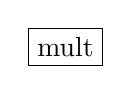
\begin{tikzpicture}[node distance = 2cm]
          \node [block] (mult) {\hs{mult}};
        \end{tikzpicture}
      };
      \node [block, right of=multset] (parityset) {
        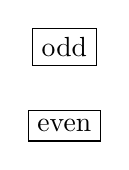
\begin{tikzpicture}[node distance = 1cm]
          \node [block]               (odd)  {\hs{odd}};
          \node [block, below of=odd] (even) {\hs{even}};
        \end{tikzpicture}
      };

      \path [line] (plusset)     -- (multset);
      \path [line] (multset)     -- (parityset);
    \end{tikzpicture}
    \caption{One possible topological sorting of simply connected components for Figure \ref{fig:dagexample} (ignoring constructors). \hs{even} and \hs{odd} are mutually recursive, no neither can appear before the other.}
    \label{fig:sccexample}
  \end{subfigure}
  \label{fig:dependencyexample}
  \caption{Sorting functions from Figure \ref{fig:haskellexample} into dependency order.}
\end{figure}

In a topological sort we say that $A < B$ for nodes $A$ and $B$ if we can reach $B$ by following edges from $A$ (if $A$ and $B$ cannot be reached from each other, their order is arbitrary). This is slightly complicated in Haskell (compared to Coq, for example), since general recursion is permitted and hence the dependency graph may contain cycles. To handle this, we use an algorithm such as Tarjan's \citep{tarjan1972depth} to produce a sorted list of \emph{strongly connected components} (SCCs), where each SCC is a mutually-recursive sub-set of the declarations (as shown in Figure \ref{fig:sccexample}). References which point to the same SCC as the expression they appear in (which includes direct recursion and mutual recursion) are given a constant feature value $f_{recursion}$.

By working through the sorted list of SCCs, storing the features of each top-level expression as they are calculated, our algorithm can be computed \emph{iteratively} rather than recursively, as shown in algorithm \ref{alg:recurrent}. This makes cyclic references particularly easy to handle: global identifiers are looked up in the current clusters $C$, and if not found the value $f_{recursion}$ is used.

\begin{algorithm}
  \begin{algorithmic}[1]
    \Require List $d$ contains SCCs of (identifier, expression) pairs, in dependency order.
    \Procedure{RecurrentCluster}{}
      \State $C  \gets []$
      \State $DB \gets \varnothing$
      \ForAll{$scc$ \textbf{in} $d$}
        \State $DB \gets DB \cup \{(i, featureVec(e)) \mid (i, e) \in scc\}$
        \State $C  \gets kMeans(DB)$
      \EndFor
      \Return $C$
    \EndProcedure
  \end{algorithmic}
  \caption{Recurrent clustering of Core expressions.}
  \label{alg:recurrent}
\end{algorithm}

As an example of this recurrent process, we can consider the Peano arithmetic functions from Figure \ref{fig:coreexample}. A valid topological ordering would be (eliding Core expressions to save space) $d = [\{(\hs{plus}, \dots)\}, \{(\hs{odd}, \dots), (\hs{even}, \dots)\}, \{(\hs{mult}, \dots)\}]$:

\begin{itemize}
  \item The first iteration through \textsc{RecurrentCluster}'s loop will set $scc \gets \{(\hs{plus}, \dots)\}$.
  \item With $i = \hs{plus}$ and $e$ as its Core expression, calculating $featureVec(e)$ is straightforward; the recursive call $\feature{\hs{plus}}$ will become $f_{recursion}$ (since \hs{plus} doesn't appear in $C$).
  \item The call to $kMeans$ will produce $C \gets [\{\hs{plus}\}]$, i.e. a single cluster containing \hs{plus}.
  \item The next iteration will set $scc \gets \{(\hs{odd}, \dots), (\hs{even}, \dots)\}$.
  \item With $i = \hs{odd}$ and $e$ as its Core expression, the call to \hs{even} will result in $f_{recursion}$.
  \item Likewise for the call to $\hs{even}$ when $i = \hs{odd}$.
  \item Since the feature vectors for \hs{odd} and \hs{even} will be identical, $kMeans$ will put them in the same cluster. The number of clusters $k = \lceil \sqrt{\lvert DB \rvert} \rceil = 2$, so the other cluster must contain \hs{plus}. Their order is arbitrary, so one possibility is $C = [\{\hs{odd}, \hs{even}\}, \{\hs{plus}\}]$.
  \item Finally \hs{mult} will be clustered. The recursive call will become $f_{recursion}$ whilst the call to \hs{plus} will become $2$, since $\hs{plus} \in C_2$.
  \item Since $k = 2$, the resulting clusters will be $C \gets [\{\hs{odd}, \hs{even}\}, \{\hs{plus}, \hs{mult}\}]$.
\end{itemize}

Even in this very simple example we can see a few features of our algorithm emerge. For example, \hs{odd} and \hs{even} will always appear in the same cluster, since they only differ in their choice of constructor names (which are discarded by $toTree$) and recursive calls (which are replaced by $f_{recursion}$). A more extensive investigation of these features requires a concrete implementation, in particular to pin down values for the parameters such as $r$, $c$, $f_{recursion}$, $\alpha$ and so on.

\subsubsection{Comparison}

Our algorithm is most similar to that of ML4PG, as our transformation maps the elements of a syntax tree to distinct cells in a matrix. In contrast, the matrices produced by ACL2(ml) \emph{summarise} the tree elements: providing, for each level of the tree, the number of variables, nullary symbols, unary symbols, etc.

There are two major differences between our algorithm and that of ML4PG: mutual-recursion and types.

The special handling required for mutual recursion is discussed above (namely, topological sorting of expressions and the $f_{recursion}$ feature). Such handling is not present in ML4PG, since the Coq code it analyses must, by virtue of the language, be written in dependency order to begin with. Coq \emph{does} have limited support for mutually-recursive functions, of the following form:

\begin{coqblock}
Fixpoint even n := match n with
                       | O   => true
                       | S m => odd m
                   end
    with odd  n := match n with
                       | O   => false
                       | S m => even m
                   end.
\end{coqblock}

However, this is relatively uncommon and unsupported by ML4PG.

The more interesting differences come from our handling (or lack thereof) for types. Coq and ACL2 are at opposite ends of the typing spectrum, with the former treating types as first class entities of the language whilst the latter is untyped (or \emph{unityped}). In both cases, we have a \emph{single} language to analyse, by ML4PG and ACL2(ml) respectively.\footnote{ML4PG can also analyse Coq's \textsc{Ltac} meta-language. Haskell has its own meta-language, Template Haskell, but here we only consider the regular Haskell which it generates.}

The situation is different for Haskell, where the type level is distinct from the value level, and there are strict rules for how they can influence each other. In particular, Haskell values can depend on types (via the type class mechanism) but types cannot depend on values.

In our initial approach, we restrict ourselves to the value level. This has several consequences:

\begin{itemize}
  \item Although they are values, we cannot distinguish between data constructors, other than using exact equality. Hence they are discarded by $toTree$.
  \item Since Core uses a single \texttt{Lam} abstraction for both value- and type-level parameters, we cannot always distinguish between them. This can cause a function's Core arity to be greater than its Haskell arity.
\end{itemize}

There is certainly promise in including types in our analysis, by pairing every term with its type as in ML4PG. This will allow fine-grained distinction of expressions which are otherwise identical, especially data constructors. Integrating types into our algorithm, and extracting them from Core expressions, is hence left as future work.
